% Mathe Formelsammlung für HM1 SoSe 2011
% 2 Seiten

% Dokumenteinstellungen
% ======================================================================	

% Dokumentklasse (Schriftgröße 6, DIN A4, Artikel)
\documentclass[6pt,a4paper]{scrartcl}

% Pakete laden
\usepackage[utf8]{inputenc}		% Zeichenkodierung: UTF-8 (für Umlaute)   
\usepackage[german]{babel}		% Deutsche Sprache
\usepackage{multicol}			% Spaltenpaket
\usepackage{amsmath}
\usepackage{amssymb}
\usepackage{esint}				% erweiterte Integralsymbole
\usepackage{multicol}			% ermöglicht Seitenspalten  
\usepackage{wasysym}			% Blitz
\usepackage{graphicx}
\usepackage[colorlinks=true, urlcolor=black]{hyperref}
  
% Seitenlayout und Ränder:
\usepackage{geometry}
\geometry{a4paper,landscape, left=6mm,right=6mm, top=0mm, bottom=3mm,includeheadfoot} 

%Kopf- und Fußzeile
\usepackage{fancyhdr}
\pagestyle{fancy}
\fancyhf{}

   \fancyfoot[C]{\textbf{Formelsammlung Relation und Funktionen} von Tim Sievers}
   \renewcommand{\headrulewidth}{0.0pt} %obere Linie ausblenden
   \renewcommand{\footrulewidth}{0.1pt} %untere Linie

   \fancyfoot[R]{Stand: \today \qquad \thepage}
	
% Schriftart SANS für bessere Lesbarkeit bei kleiner Schrift
\renewcommand{\familydefault}{\sfdefault} 


% Custom Commands
\renewcommand{\thesubsection}{\arabic{subsection}}
\newcommand{\me}[1]{\ensuremath{\left\{#1\right\}}}
\newcommand{\dme}[2]{\ensuremath{\left\{#1\,\vert\,#2 \right\}}}
\newcommand{\abs}[1]{\ensuremath{\left\vert#1\right\vert}}
\newcommand{\un}[1]{\; \unit{#1} }
\newcommand{\unf}[2]{\;\left[ \unitfrac{#1}{#2} \right]}
\newcommand{\norm}[2][\relax]{\ifx#1\relax \ensuremath{\left\Vert#2\right\Vert}\else \ensuremath{\left\Vert#2\right\Vert_{#1}}\fi}
\newcommand{\enbrace}[1]{\ensuremath{\left(#1\right)}}
\newcommand{\nira}[1]{\ensuremath{\overset{n \rightarrow \infty}{\longrightarrow}}}
\newcommand{\os}[2]{\ensuremath{\overset{#1}{#2}}}
\makeatletter
\newcommand{\R}{\mathbb{R}}
\newcommand{\Ra}[0]{\ensuremath{\Rightarrow}}
\newcommand{\ra}[0]{\ensuremath{\rightarrow}}
\newcommand{\gk}[1]{\ensuremath{\left\lfloor#1\right\rfloor}}
\newcommand{\sprod}[2]{\ensuremath{%
  \setbox0=\hbox{\ensuremath{#2}}
  \dimen@\ht0
  \advance\dimen@ by \dp0
  \left\langle #1\rule[-\dp0]{0pt}{\dimen@},#2\right\rangle}}
  
%Custom functions
\DeclareMathOperator{\arccot}{arccot}
\DeclareMathOperator{\Bild}{Bild}
\DeclareMathOperator{\diag}{diag}
\DeclareMathOperator{\rg}{rg}


% Dokumentbeginn
% ======================================================================
\begin{document}
%\section{}
% ----------------------------------------------------------------------

% Aufteilung in Spalten
\begin{multicols*}{2}

\subsection{Relationen}
\subsubsection{Definitionen der Eigenschaften}
\begin{tabular}{lll}
R linkstotal	    & Jedes Element x steht mit mindestens einem Element y in Relation.								\\
& $\forall$x $\exists$y : (x, y) $\in$ R \\
R rechtstotal		& Für jedes Element y existiert mindestens ein Element x, das mit y in Relation steht.				\\
& $\forall$y $\exists$x : (x, y) $\in$ R \\
R linkseindeutig	& Keine zwei verschiedenen Elemente $x_1$ und $x_2$ stehen mit dem selben Element y in Relation.	\\
& $\forall x_1$ $\forall x_2$ $\forall y$ : ( ($x_1$, $y$) $\in$ R $\land$ ($x_2$, $y$) $\in$ R $\Rightarrow$ ($x_1 = x_2$) ) \\
R rechtseindeutig	& Kein Element x steht mit zwei verschiedenen Elementen $y_1$ und $y_2$ in Relation.				\\
& $\forall$x $\forall y_1$ $\forall y_2$ : ( (x, $y_1$) $\in$ R $\land$ (x, $y_2$) $\in$ R $\Rightarrow$ ($y_1$ = $y_2$) ) \\
R reflexiv			& Jedes Element x steht mit sich selbst in Relation.												\\
& $\forall$x : (x, x) $\in$ R \\
R irreflexiv	    & Kein Element x steht mit sich selbst in Relation												\\
& $\forall$x : (x, x) $\notin$ R $\Leftrightarrow$ $\lnot\exists$x : (x, x) $\in$ R \\
R symmetrisch		& Wenn x mit y in Relation steht, dann steht auch y mit x in Relation.							\\
& $\forall$x $\forall$y : ( (x, y) $\in$ R $\Rightarrow$ (y, x) $\in$ R ) \\
R asymmetrisch		& Wenn x mit y in Relation steht, dann steht y nicht mit x in Relation.							\\
& $\forall$x $\forall$y : ( (x, y) $\in$ R $\Rightarrow$ (y, x) $\notin$ R ) \\
R antisymmetrisch	& Wenn x mit y und y mit x in Relation stehen, dann sind x und y identisch.						\\
& $\forall$x $\forall$y : ( (x, y) $\in$ R $\land$ (y, x) $\in$ R $\Rightarrow$ (x = y) ) \\
R transitiv			& Wenn x mit y und y mit z in Relation stehen, dann steht auch x mit z in Relation.				\\
& $\forall$x $\forall$y $\forall$z : ( (x, y) $\in$ R $\land$ (y, z) $\in$ R $\Rightarrow$ (x, z) $\in$ R ) \\
\end{tabular}

\subsubsection{Beweisen der Eigenschaften (Beispiel 1)}
Welche der Eigenschaften linkstotal, rechtstotal, linkseindeutig, rechtseindeutig, irreflexiv,\\
symmetrisch, antisymmetrisch, transitiv hat die folgende Relation Rel auf der Menge\\
R der reellen Zahlen, und welche hat sie nicht?\\
Rel = $\{ (x, y) \in \mathbb{R} \times \mathbb{R} | x \cdot y = –1 \}$\\
Beweisen Sie jede Ihrer Behauptungen.\\
\\
Lösung (Kurzform):\\
\textbf{Nicht linkstotal/rechtstotal}: Für x = 0 gibt es kein y mit $x \cdot y$ = –1 und umgekehrt.\\
\textbf{Links-/rechtseindeutig}: Wenn die Auflösung nach x oder y möglich ist, ist sie eindeutig.\\
\textbf{Irreflexiv}: $x^2$ = –1 kann für kein reelles x gelten.\\
\textbf{Symmetrisch}: klar.\\
\textbf{Nicht antisymmetrisch}: klar.\\
\textbf{Nicht transitiv}: Gegenbeispiel: x = 2, y = –1/2, z = 2.\\

\subsubsection{Beweisen der Eigenschaften (Beispiel 2)}
Welche der Eigenschaften linkstotal, rechtstotal, linkseindeutig, rechtseindeutig, irreflexiv,\\
symmetrisch, antisymmetrisch, transitiv hat die folgende Relation Rel auf der Menge\\
R der reellen Zahlen, und welche hat sie nicht?\\
Rel = $\{ (x, y) \in \mathbb{Z} \times \mathbb{Z} | x \cdot y < 1 \}$\\
Beweisen Sie jede Ihrer Behauptungen.\\
\\
Lösung (Kurzform):\\
\textbf{linkstotal/rechtstotal}: Für beliebiges x wähle y = 0 und umgekehrt.\\
\textbf{Nicht Links-/rechtseindeutig}: klar.\\
\textbf{Nicht Irreflexiv}: (0, 0) $\in$ Re.\\
\textbf{Symmetrisch}: Für alle x und alle y gilt $x \cdot y = y \cdot x$.\\
\textbf{Nicht antisymmetrisch}: klar.\\
\textbf{Nicht transitiv}: Gegenbeispiel: x = 1, y = –2, z = 3.\\

\subsubsection{Äquivalenzklassen (allgemein)}
Eine Relation R $\subseteq$ A $\times$ A heißt genau dann Äquivalenzrelation, wenn sie reflexiv, symmetrisch und transitiv ist.\\
Gilt (x,y) $\in$ R , so sagt man, x ist äquivalent zu y (unter R).\\


\subsubsection{Äquivalenzklassen (Beispiel)}
Auf der Menge Z der ganzen Zahlen sei die folgende Relation Rel definiert:\\
Rel := $\{ (x, y) \in Z \times Z | 5$ teilt (x + 4y) \}\\
a) Beweisen oder widerlegen Sie, dass diese Relation eine Äquivalenzrelation ist.\\
b) Falls Rel eine Äquivalenzrelation ist, dann geben Sie alle Äquivalenzklassen von\\
Rel an.\\
\\
Lösung:\\
a) Vorbetrachtung: 5 teilt (x + 4y)  5 teilt (x – y), denn es wird die durch 5 teilbare\\
Zahl 5y subtrahiert.\\
Man kann Rel also auch wie folgt charakterisieren:\\
Rel := $\{ (x, y) \in Z \times Z | 5$ teilt (x + 4y) \}\\
reflexiv: (x, x) $\in$ Rel, denn (x – x) = 0 ist Vielfaches von 5;\\
symmetrisch: 5 teilt (x – y) $\Leftrightarrow$ 5 teilt (y – x);\\
transitiv: 5 teilt (x – y) und 5 teilt (y – z) $\Rightarrow$ 5 teilt (x – z) (Summe).\\
$\Rightarrow$ Rel ist Äquivalenzrelation.\\
b) Rel erzeugt vier Äquivalenzklassen A0, A1, A2, A3 und A4: Ak enthält genau die\\
ganzen Zahlen, die bei Division durch 5 den Rest k ergeben.\\
\\

\subsection{Funktionen}

\subsubsection{Horner Schema:}
Beispiel: $x^4$ - $x^3$ - $3x^2$ + 5x -2 = 0\\
Hinweis zum Finden einer Lösung: Nur Koeffizienten betrachten, sollte das 0 ergeben, dann ist 1 eine Lösung:\\
$1 - 1 -3 + 5 - 2 = 0$\\
Damit dann das Horner Schema abarbeiten\\
Schematisch:\\
$ax^3 + bx^2 + cx + d = 0$, mit möglicher Lösung x=n\\
\begin{tabular}{r|rrrrl}
	& a 				& b 		& c 			& d &\\
n 	& $\downarrow$	& na 	& n(b+na) 	& n(c+n(b+na)) &\\
\hline
 	& a 				& b+na 	& c+n(b+na) 	& 0 & $\leftarrow$(sollte 0 sein, damit es aufgeht)\\
\end{tabular}\\
Danach hat man eine neue Lösung mit veringertem Exponenten. Darauf kann man dann wieder das Hoener Schema anwenden oder direkt die pq-Formel.\\
Am obigen Beispiel betrachtet:\\
\begin{tabular}{r|rrrrr}
	& 1 				& -1 & -3 & 5  & -2\\
1 	& $\downarrow$	& 1 	 & 0  & -3 & 2\\
\hline
 	& 1 				& 0 	 & -3 & 2 & 0\\
\end{tabular}\\
Das ergibt: $x^3 + 0x^2 -3x +2 = 0$\\
Hierfür wieder eine Nullstelle erraten (kann die gleiche sein wie eben), und wieder das HS anwenden:\\
\begin{tabular}{r|rrrrr}
	& 1 				& 0 & -3 & 2\\
1 	& $\downarrow$	& 1 	& 1  & -2\\
\hline
 	& 1 				& 1 	& -2 & 0\\
\end{tabular}\\
Ergibt also: $1x^2 + 1x -2 = 0$\\
Und das lässt sich nun mit pq-Formel lösen.\\

\subsubsection{Definitionsbereich etc.}
Definitionsbereich bei Brüchen: alles außer den Stellen wo der Nennen 0 wäre \\
Definitionsbereich bei Wurzeln: alles wo unter der Wurzel etwas $\geq$ 0 steht \\
Definitionsbereich bei Exponenten: egal, ganz $\mathbb{R}$ \\
Definitionsbereich bei Logarithmen: der Numerus (das x bei ln(x)) muss $>$ 0 sein \\
Definitionsbereich ohne z.B. die 1: $\mathbb{D} = \mathbb{R} \backslash \{1\}$ \\

\subsubsection{Ableitungen}
\begin{tabular}{ll}
Konstantenregel						& $ c'=0 $																								\\
Faktorregel							& $ (c \cdot u(x))' = c u'(x) $																			\\
Potenzregel							& $ \left(u^n\right)' = n \cdot u^{n-1} \cdot u'\; (n \in \mathbb R, \; n \neq 0) $						\\
Summenregel							& $ (u\pm v)' = u'\pm v' $																				\\
Produktregel für zwei Funktionen		& $ (uv)' = uv'+u'v $																					\\
Produktregel für drei Funktionen		& $ (uvw)' = uvw' + uv'w + u'vw $																		\\
Produktregel für $ N $ Funktionen	& $ (u_1u_2...u_N)' = \sum_{i=1}^Nu_1...u_i'...u_N $														\\
Quotientenregel						& $ \left(\frac{u}{v}\right)' = \frac{vu'-uv'}{v^2}, \; \left( \frac{1}{v}\right)' = \frac{-v'}{v^2} $		\\
Kettenregel für zwei Funktionen		& $ \frac{\rm d u}{\rm d x} = \frac{\rm d u}{\rm d v}\cdot \frac{\rm d v}{\rm d x} $ für $ u(v(x)) \Leftrightarrow u'(v(x)) \cdot v'(x)$		\\
Kettenregel für drei Funktionen		& $ \frac{\rm d u }{\rm d x} = \frac{\rm d u}{\rm d v}\cdot \frac{\rm d v}{\rm d w}\cdot \frac{\rm d w}{\rm d x} $ für $ u(v(w(x))) $ \\
\end{tabular}\\
\\
\textbf{Regeln:}\\
\begin{tabular}{l|l|l}
$ y=f(x) $		& $ y'=f'(x) $ 								& Einschränkungen 									\\
\hline
$ c $(const.)	& 0 																								\\	
$ x $			& 1																								\\
$ x^n $			& $ n \cdot x^{n-1} $						& $ n \in \mathbb N \setminus \{0\} $ 				\\
$ x^r $			& $ r \cdot x^{r-1} $						& $ r \in \mathbb R, \; r \neq 0, x>0 $ 				\\
$ \sin x $		& $ \cos x $ 								& sin $\rightarrow$ cos $\rightarrow$ -sin $\rightarrow$ -cos $\rightarrow$ sin\\	
$ \cos x $		& $ -\sin x $ 								&													\\
$ \tan x $		& $ 1+ \tan^2 x = \frac{1}{\cos^2 x} $		& $ x \neq (2k+1)\frac{\pi}{2}, \; k \in \mathbb Z $ 	\\
$ \cot x $		& $ -(1+ \cot^2 x) = - \frac{1}{\sin^2 x} $	& $ x \neq k \pi, \; k \in \mathbb Z $ 				\\
$ a^x $			& $ a^x \ln a $								& $ a>0 $ 											\\
$ \rm e^x $		& $ \rm e^x $ 								&													\\	
$ \ln x $		& $ \frac{1}{x} $							& $ x>0 $ 											\\
$ \log_a x $		& $ \frac{1}{x \ln a} $						& $ a>0, \; a \neq 1; \; x>0 $ 						\\
\end{tabular}

\subsubsection{Kurvendiskussion}

\textbf{Symmetrie:}\\
Achsensymmetrie: f(x) = f(-x) (alle Exponenten von x sind gerade)\\
Punktsymmetrie: f(x) = -f(-x) (alle Exponenten von x sind ungerade)\\
\\
\textbf{Nullstellen:}\\
f(x) = 0 und dann ausrechnen\\
Strategien:\\
- x ausklammern, wenn x überall auftaucht. Dann ist x=0 eine Lösung und das was die Klammer = 0 setzt\\
- eine Nullstelle durch Probieren ermitteln und dann Polinomdivision\\
- z.B. $x^2$ durch z ersetzen und dann pq-Formel\\
\\
Bedeutung von Nullstellen:\\
Einfach Nullstelle: Kurve kreuzt die Achse\\
doppelte Nullstelle: Extremwert (Hoch- oder Tiefpunkt)\\
dreifache Nullstelle: Sattelpunkt\\
\\
Eine hebbare Lücke liegt dort vor wo der im Nenner und gleichzeitig im Zähler eine Nullstelle vorliegt. Also nur bei gebrochenrationalen Zahlen.\\
\textbf{Schnitt mit y-Achse:}\\
x = 0, also f(0) berechnen\\
\\
\textbf{Extremwerte:}\\
Ein lokales Minimum ist dort wo die 1. Ableitung = 0 ist und die 2. Ableitung $\neq$ 0\\
f^{\prime}(x) = 0 $\land$ f^{\prime\prime} $\neq$ 0\\
wenn $f^{\prime\prime}(x) < 0$ dann ist es ein Hochpunkt (lokales Maximum)\\
 wenn $f''(x) > 0$ dann ist es ein Tiefpunkt (lokales Minimum)\\
\\
Ein Wendepunkt liegt dort wo die 2. Ableitung = 0 und die 3. Ableitung $\neq$ 0 ist\\
f^{\prime\prime}(x) = 0 $\land$ f^{\prime\prime\prime}(x) $\neq$ 0\\
\\
\textbf{Verhalten im Unendlichen:}\\
Hier geht es darum zu schauen wie sich f(x) bei x $\rightarrow$ +unendlich und bei x $\rightarrow$ -unendlich verhält.\\
Dazu beachten ob die Exponenten von x gerade oder ungerade sind!\\
\\
Andere Option: Asymptote berechnen\\
Bei gebrochen rationalen Funktionen kann man den Bruch durch Polinomdivision berechnen und erhält evtl. eine Konstante und einen Rest der anzeigt wo sich die Funktion annähert.\\
\\
\textbf{Skizze:}\\
- Nullstellen einzeichnen\\
- Schnitt mit der y-Achse einzeichnen\\
- Extremwerte einzeichnen\\
- Wendepunkte einzeichnen\\
- Hoch- und Tiefpunkte schon mal andeuten\\
- dann die Kurven durchziehen\\
\\
\textbf{Wertebereich:}\\
Den kann man dann in der Skizze ablesen. Sprich man betrachtet ob es eine Asymptote im Negativen oder im Positiven gibt. Diese begrenzen dann den Wertebereich. Am Ende kommt dann z.B. sowas raus: $\mathbb{W} = [-4; \infty)$
\subsection{Diverses}
- Logarithmusregeln
- Potenzregel

\subsection{Allgemeine Hilfsmittel}
\subsubsection{P-Q-Formel}
$
x^2 + p\cdot x + q = 0\\
{x}_{1,2} = \frac{-p}{2} \pm \sqrt{(\frac{p}{2})^2 - q}
$
\subsubsection{Binomische Formeln}
Erste binomische Formel $(a+b)^{2}=a^{2} + 2ab + b^{2}$ \\
Zweite binomische Formel $(a-b)^{2}=a^{2} - 2ab + b^{2}$ \\
Dritte binomische Formel $(a+b)\cdot (a-b)=a^{2}-b^{2}$ \\


\subsubsection{verschiedene Winkel}
\begin{tabular}{lll}
$\alpha^\circ$&rad($\alpha$)&$\cos{\alpha}$\\
\hline
\\
$0^\circ$ & 0 & 1 \\
\\
\hline
\\
$30^\circ$  & $\frac{1}{6}\pi$  & $\frac{1}{2}\sqrt{3}$ \\
\\
\hline
\\
$45^\circ$  & $\frac{1}{4}\pi$  & $\frac{1}{2}\sqrt{2}$ \\
\\
\hline
\\
$60^\circ$  & $\frac{1}{3}\pi$  & $\frac{1}{2}$ \\
\\
\hline
\\
$90^\circ$  & $\frac{1}{2}\pi$  & $0$ \\
\\
\hline
\\
$120^\circ$ & $\frac{2}{3}\pi$  & $-\frac{1}{2}$ \\
\\
\hline
\\
$135^\circ$ & $\frac{3}{4}\pi$  & $-\frac{1}{2}\sqrt{2}$ \\
\\
\hline
\\
$150^\circ$ & $\frac{5}{6}\pi$  & $-\frac{1}{2}\sqrt{3}$ \\
\\
\hline
\\
$180^\circ$ & $\pi$             & $-1$ \\
\\
\hline
\\
$210^\circ$ & $\frac{7}{6}\pi$  & $-\frac{1}{2}\sqrt{3}$ \\
\\
\hline
\\
$225^\circ$ & $\frac{5}{4}\pi$  & $-\frac{1}{2}\sqrt{2}$ \\
\\
\hline
\\
$240^\circ$ & $\frac{4}{3}\pi$  & $-\frac{1}{2}$ \\
\\
\hline
\\
$270^\circ$ & $\frac{3}{2}\pi$  & $0$ \\
\\
\hline
\\
$300^\circ$ & $\frac{5}{3}\pi$  & $\frac{1}{2}$ \\
\\
\hline
\\
$315^\circ$ & $\frac{7}{4}\pi$  & $\frac{1}{2}\sqrt{2}$ \\
\\
\hline
\\
$330^\circ$ & $\frac{11}{6}\pi$ & $\frac{1}{2}\sqrt{3}$ \\
\\
\hline
\\
$360^\circ$ & $2\pi$            & $1$ \\
\end{tabular}

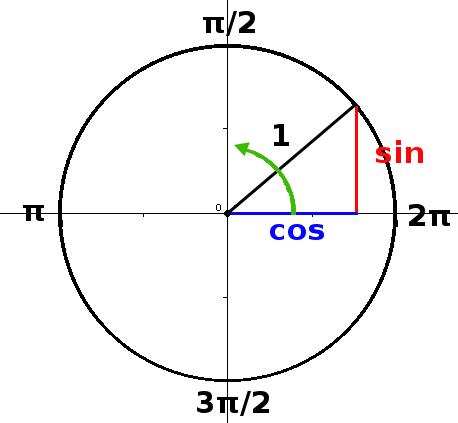
\includegraphics[width=150px]{einheitskreis1.png}

\end{multicols*}
% Ende der Spalten


% Dokumentende
% ======================================================================
\end{document}